
\documentclass{article}[12pt]
%Required: You must have these
\usepackage{graphicx}
\usepackage{tabularx}
\usepackage{natbib}
%\usepackage{caption}
%\usepackage{subcaption}
\usepackage{array}
\usepackage{amsmath}
%\usepackage[backend=bibtex]{biblatex}
\setkeys{Gin}{width=0.8\textwidth}
%\setlength{\captionmargin}{30pt}
\setlength{\abovecaptionskip}{10pt}
\setlength{\belowcaptionskip}{10pt}
\topmargin -1.5cm 
\oddsidemargin -0.04cm 
\evensidemargin -0.04cm 
\textwidth 16.59cm
\textheight 23.94cm 
\parskip 7.2pt 
\renewcommand{\baselinestretch}{1.1} 	
\parindent 0pt

\bibliographystyle{refs/styles/newphyto.bst}
\usepackage{Sweave}
\begin{document}
\Sconcordance{concordance:prief_outline.tex:prief_outline.Rnw:%
1 2 1 1 0 47 1}


\section{Introduction}
Phenology, the timing of seasonal life cycle events is cool/important. Even (plant) species with similar growth forms, habitat requirements and environmental tolerance can express markedly different phenology.  There is an emerging consensus based on short-term experiments manipulating the germination phenology of seeds, that differences in relative phenology among species is a strong mediator of species interactions \citep{}. Precocious relative germination phenology, functions as a seasonal priority effect  \citep{Wainwright_2011, Buonaiuto2021}, allowing early-active species to access limited seasonal resources and modify the growth environment before competitors emerge \citep{Kardol2013}. 

Theory suggests that these seasonal priority effects, may play an important role in maintaining species coexistence, serving as a stabilizing (or equalizing?) mechanism between species with different intrinsic competitive abilities (ie weaker competitors germinate first). At an the extreme, precocious germination could also allow can allow weaker competitors to competitively exclude stronger ones--- a trait which of often invoked to explain the success of invasive plants, many of which germinate rapidly and early in the growing season \citep{Gioria2018,Gioria:2017wo}.

However, this suggested link between seasonal priority effects and long-term coexistence is, at present, highly speculative, relying on extrapolation of within-season competition proxies, or at best, short-term study results that isolate germination phenology from the climactic cues that control germination timing in most natural systems. 

Here, using examples from empirical germination assays, we highlight that it is this dependency between germination phenology and the environment that make it feasible that priortiy effects matter and also tenuous to ascribe seasonal priority effects as an important mechanism of long term coexistence, and emphasize that linking climatic variation and seasonal priority effects is critical for forecasting how ecological communities will change under future climate change.

With this foundation, we then used sexy, awesome models to do stuff, and address our questions.

\section*{Seasonal Priorty Effects are dependent on seasonal environmental variation}

In most ecological systems, seed germination is under strong environmental control. In arid ecosystems water matters. In other temperate and boreal systems, chilling matters. Species vary in there sensitivity to the factors. These factors also vary. Therefore seasonal priority effects are the manifestation of the interaction between sensitivity to the environment ( a species-level trait) and the environment itself. This means that interannual variation in environment strongly influences the strength of the seasonal priorty effect.

To better understand these dynamics, we performed a series of germination assays with regionally co-occuring herbaceous species under varying chilling and incubation conditions. We used these studies to estimate species level sensitivies to these environmental cues, and forecast phenological differences among species under difference climate conditions (see Supplemental Methods.)

From these trials we see three things. Species have different sensitivities to the same cues (Fig. \ref{Fig:emp}. This was true for species with the same dormancy class, closely related species and those in the same habitat (Make Supplemental figure.)

In general, at higher levels of chilling, the sensitivity differences reduced the realized differenences in germination phenology amoung species and lower levels increased them. (Fig. \ref{Fig:surv}). Incubations temperature were interesting becuase species crossthed the optimum (Fig. \ref{Fig:emp}), which also made it that cooler temps standardize phenology (Fig. \ref{Fig:surv}). One thing this means is that species with similar and different sensitives can express different and similar phenology. For example the species in Fig. \ref{Fig:case}. (I'd potentially like to develop this into a ``box").

This also suggests something else. Layout tradeoff theory here. Under a stable environment coexistence could be achieved through a trade off. If that shifts the trade off should shift.


but this is hard to study .Of course the biggest challenge is we cannot observe coexistence. Explain the experiments, most experiments manipulate the SPE directly by sequential planting, that means even in experiments last for multiple seasons, the priority effect is only applied once (decide where to talk about this). Other unrealism of this approach discussed in our previous paper.

The tradeoff between competition and phenology is hard to measure. Models that link all these things can help.

%Even isolating the phenological sensitivity is lacking. Most germination studies dont fit curves, just biany or threshhold effects.





%Species have different sensitivity to environmental cues (Fig 1a), which manifests in different patterns of phenological assembly under different conditions, species with similar sensitivies can manifest strongly different effects under some conditions, and species with different sensitives can converge. This mean 

%A second complexity is germination phenology isnt the only aspect the at dependent on the environment. The number of seeds that germination affect this dynamics too. Complexisty


\section{Models to the rescue}
Models can define sensitivy and competitive ability. Can isolate germination phenology from other germination responses and simulate long term dynamics and environmental change. We modified a model to coexistence to do this.

Paragraoh in the approach

\section{Coexistice and competitive exclusion under alternative climate scenario}
Under both high and low chill scenarios, coexistence happened due to a tradeoff. The slope got steeper and coexistence less frequencies with lower chilling (Fig. \ref{Fig:coexistence}). Cases where the stronger competitor (lower Rstar) was extripated due to phenological differences also occured in both scenarion. Slope didn't change, but the frequency did.

Fig. \ref{Fig:differences} explain both of these phenomena.


\section{A path forward}
Models are still over simplifications. We can improve experiments and stuff.
\begin{enumerate}
\item Germination phenology as a response curve
\item spaital variability chillnig could go up or down
\item Experiments with seasonal cary-over
\item seasonal priort effects and other germinations variation

\end{enumerate}
\pagebreak
\section*{Figures}
\begin{figure}[h!]
  \centering
 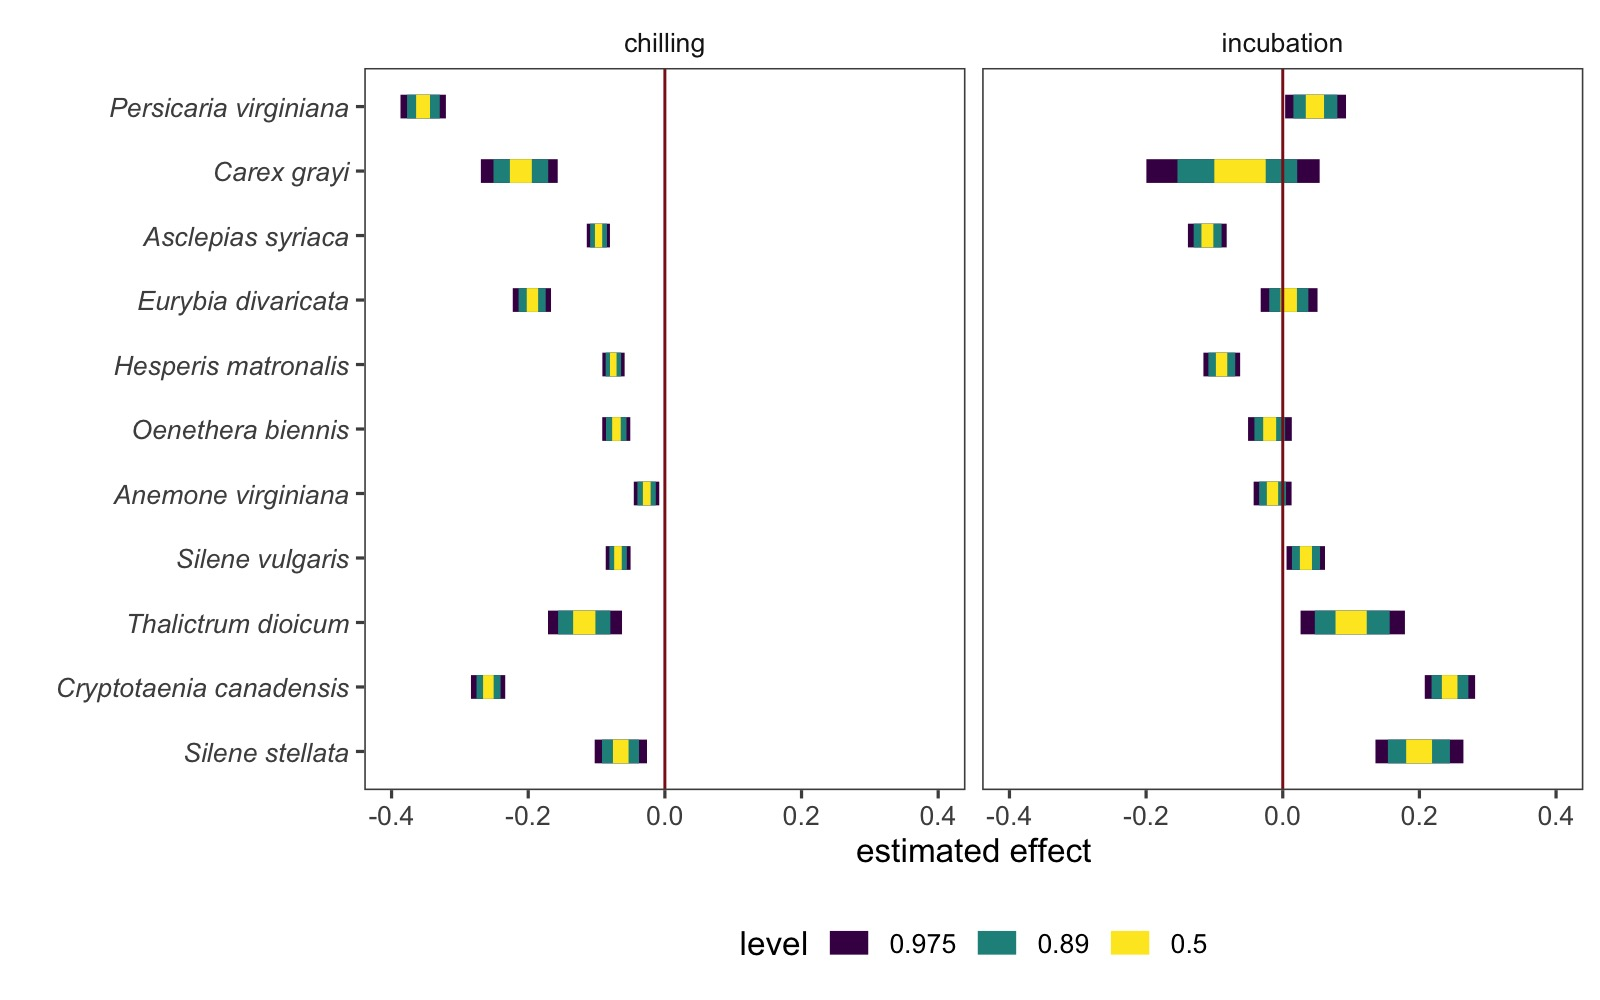
\includegraphics[width=\textwidth]{..//plots/mus_survival.jpeg}
    \caption{Co-occuring species differ in their sensitivity to environmental variation. Describe plot}
    \label{Fig:emp}
\end{figure}


\begin{figure}[h!]
  \centering
 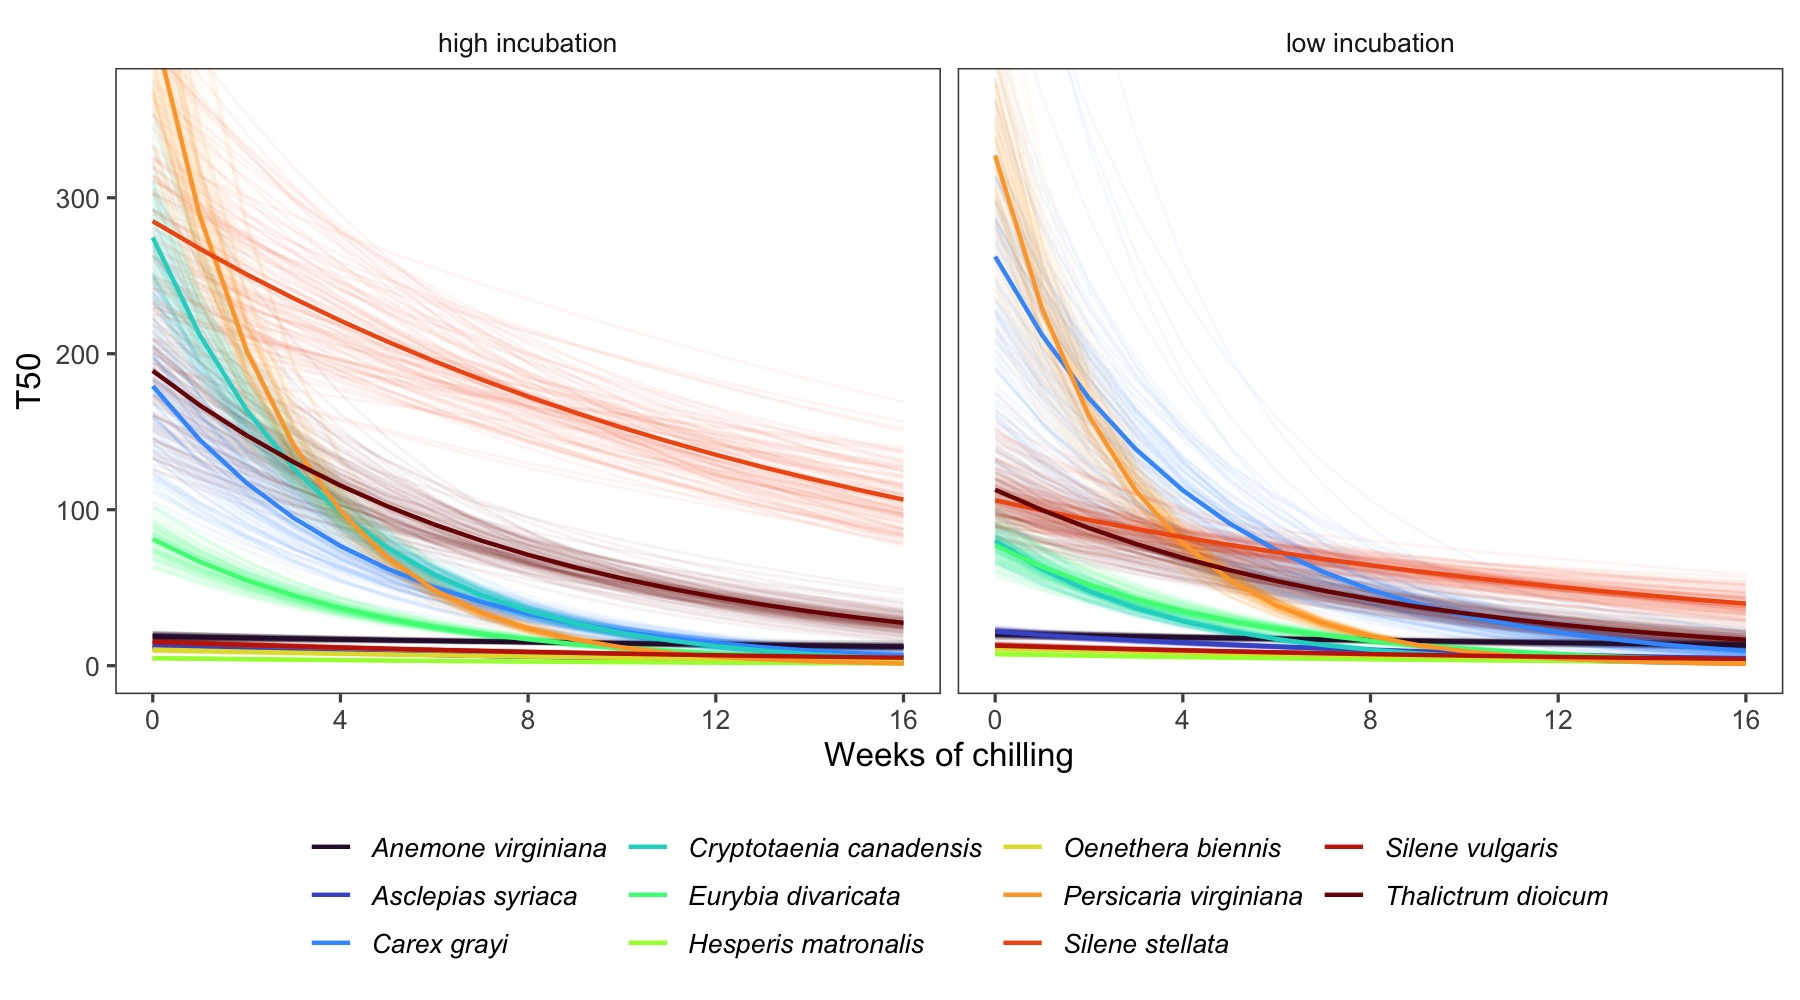
\includegraphics[width=\textwidth]{..//plots/surv_prieff.jpeg}
    \caption{Differences in phenological sensitivity among species are minimized at high chill/low incubations temperatures.}
    \label{Fig:surv}
\end{figure}


\begin{figure}[h!]
  \centering
 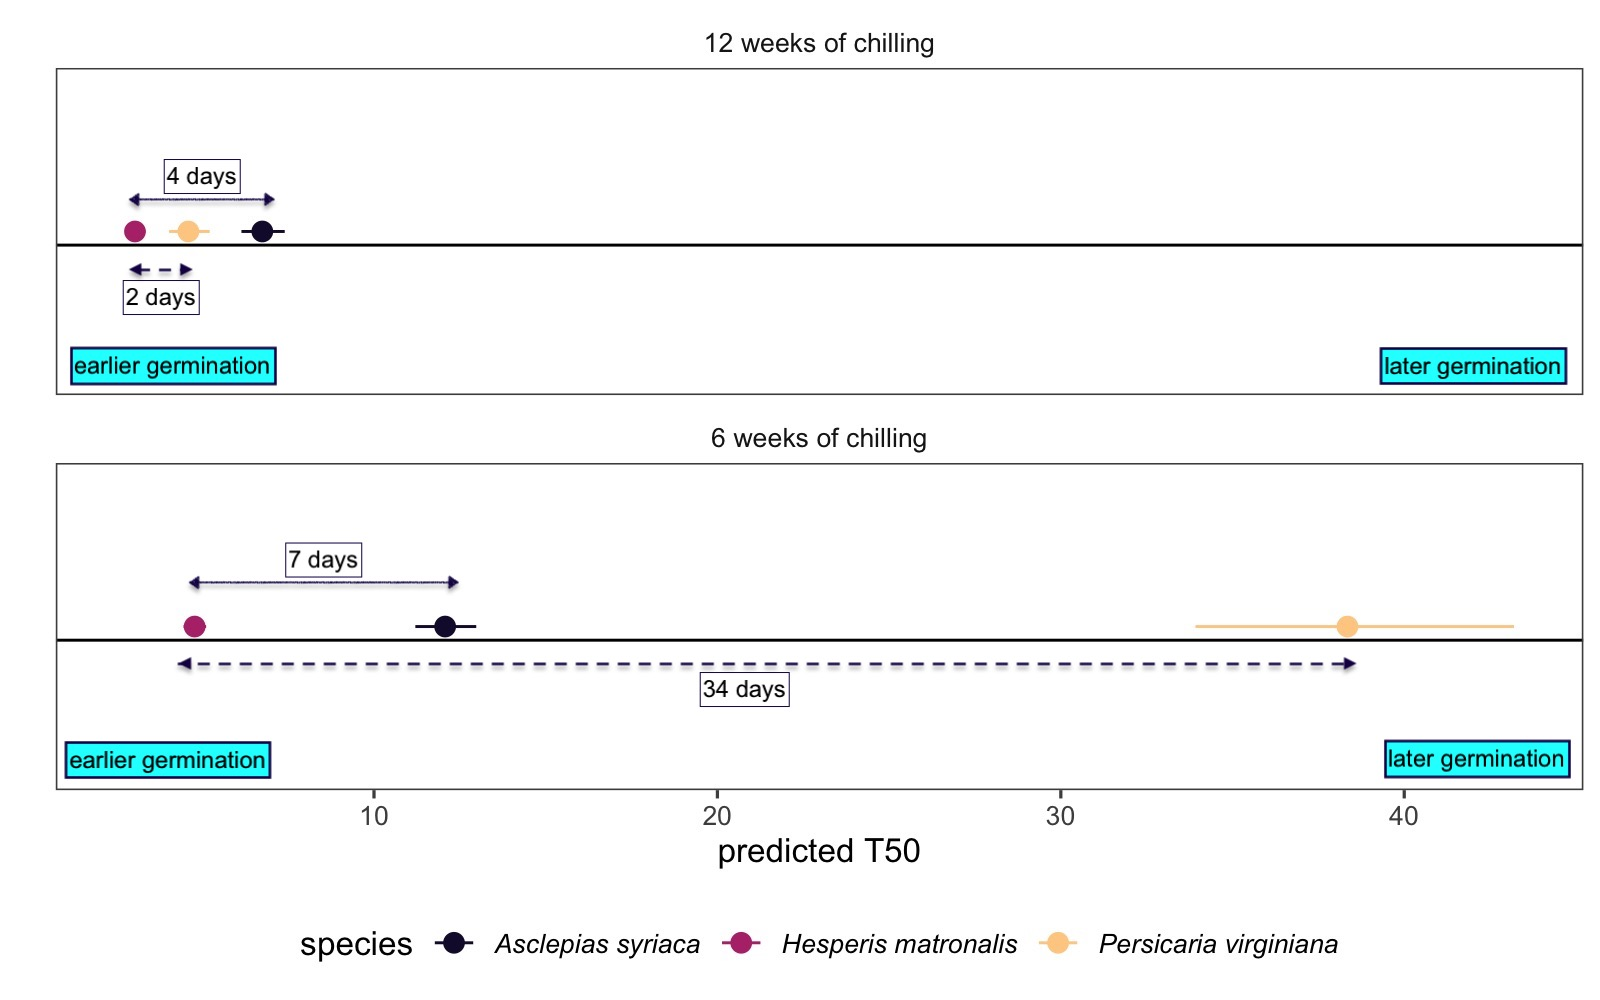
\includegraphics[width=\textwidth]{..//plots/sps_case_examps.jpeg}
    \caption{Environmental variation can both increase the difference in germination phenology for species with similar environmental sensitivity (\emph{Hesperis matronalis} vs. \emph{Asclepias syriaca}) and decrease the difference in germination phenology for species with contrasting levels of sensitivity (\emph{Hesperis matronalis} vs. \emph{Persicaria virginiana}). Description of what this plot is. Generally high levels of chilling minimize germination differences amoung species while lower levels of chilling enhance differences.}
    \label{Fig:case}
\end{figure}


\begin{figure}[h!]
  \centering
 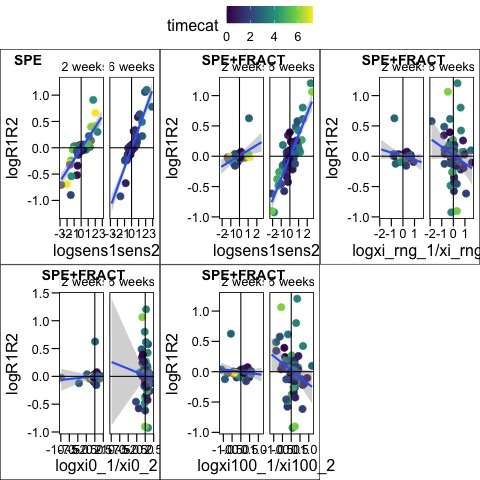
\includegraphics[width=\textwidth]{..//plots/coexistance_runner.jpeg}
    \caption{Reduced chilling shifts the slope of the coexistence tradeoff between priority effects and competitive ability, reduces frequency that coexistence occurs and increase the frequencey that stronger competitor are exptripated due to phenological differences.}
    \label{Fig:coexistence}
\end{figure}


\begin{figure}[h!]
  \centering
 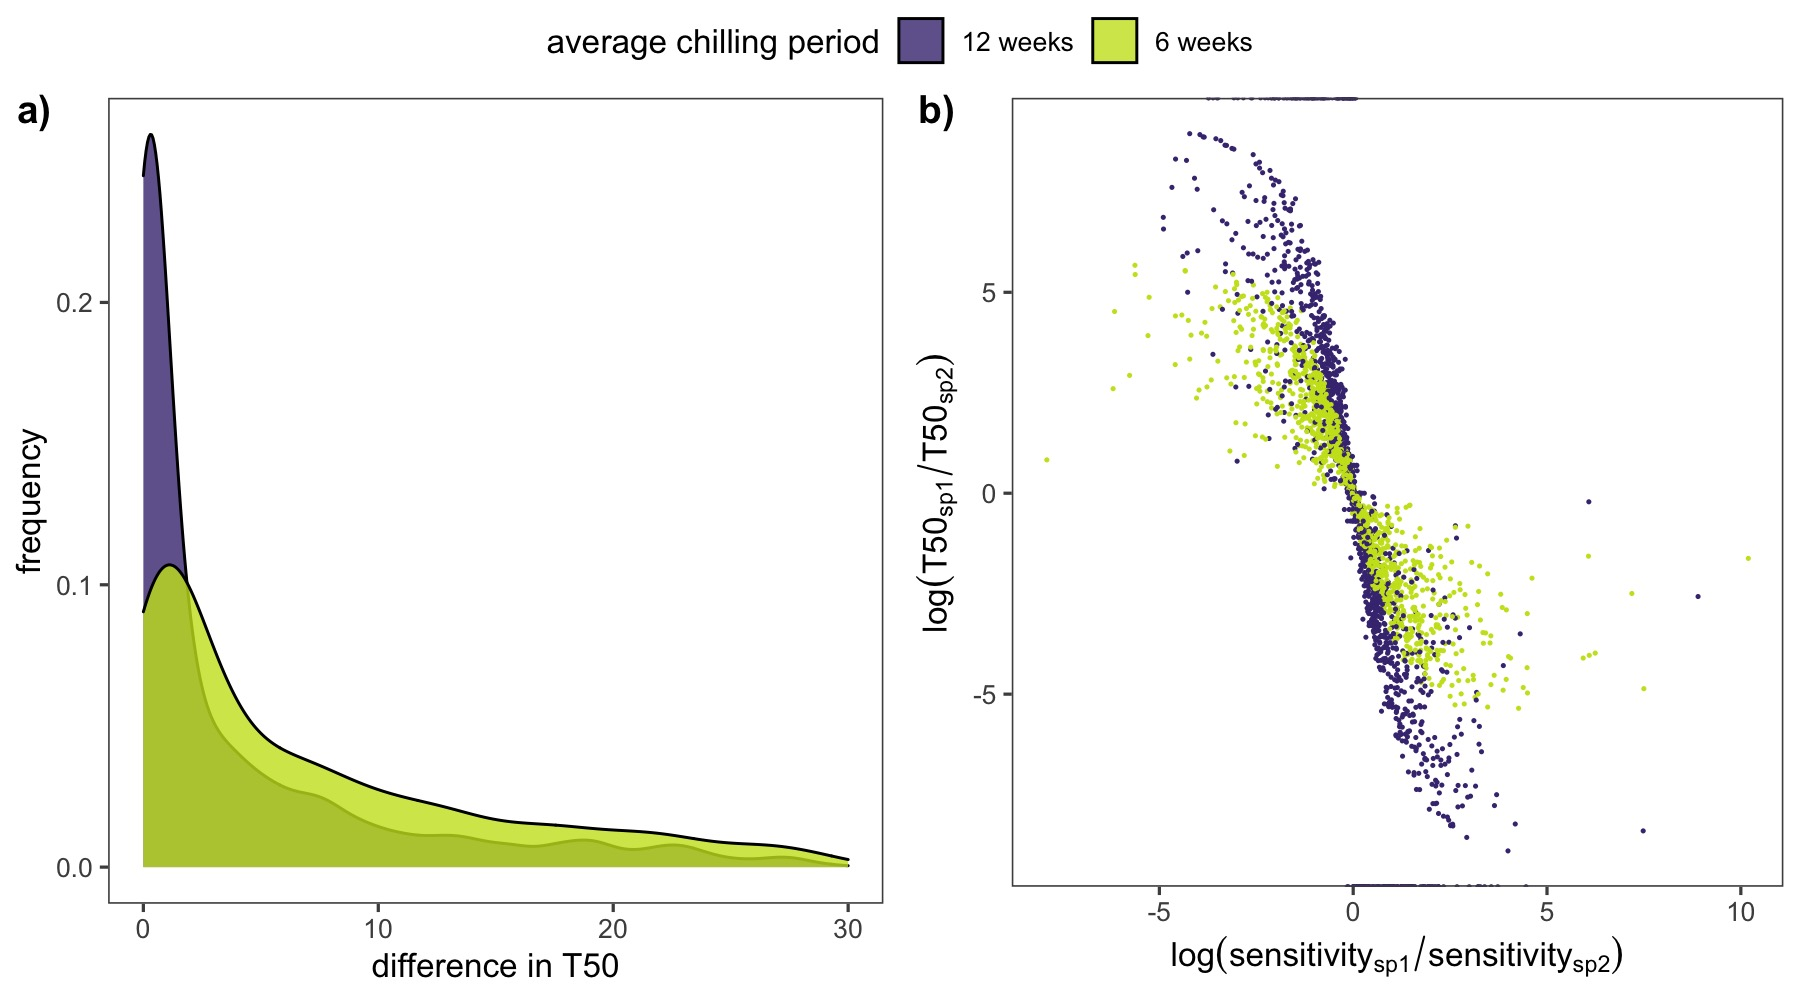
\includegraphics[width=\textwidth]{..//plots/coexistance_chilldiffs.jpeg}
    \caption{Under high chilling, species frequently germination closer together  than under lower chilling conditions (a). This environmental variation also alters the relationship between inherent sensitivity differences amoung species and realized differences in germination phenology (b). This explains patterns in Fig. \ref{Fig:coexistence}.}
    \label{Fig:differences}
\end{figure}


\end{document}
